\documentclass[spanish,mexico]{article}
\usepackage[table,xcdraw]{xcolor}
\usepackage[utf8]{inputenc}
%\usepackage[table,xcdraw]{xcolor}
\PassOptionsToPackage{hyphens}{url}\usepackage{hyperref}
%\usepackage[table,xcdraw]{xcolor}
\usepackage[italicdiff]{physics}
\usepackage{babel}
\usepackage{amsthm, amssymb, amsmath, amsfonts, bbm, mathtools}
\usepackage{csquotes}
\usepackage{enumerate}
\usepackage[shortlabels]{enumitem}
\usepackage{titling}
\usepackage{ wasysym }
\usepackage{lmodern} %optimiza algunas fuentes
\usepackage{float}
\usepackage{mathrsfs}
\usepackage{dsfont}
\usepackage{listings}
\decimalpoint
\usepackage[margin=1in]{geometry}
\usepackage[shortlabels]{enumitem}
%\usepackage[dvipsnames]{xcolor}
% \usepackage[pass,showframe,margin=1in]{geometry}
% \usepackage{layout} %use \layout
\usepackage{tikz}
\usepackage{algorithm}
\usepackage{algpseudocode}




%Ref
%\usepackage[capitalise]{cleveref}
% \usepackage{biblatex}
% \addbibresource{ref.bib}
\usepackage{hyperref}

%Imagenes
\usepackage{caption} %para usar caption con *
% \usepackage{svg} %inserta imagenes svg
% \svgpath{{./imgs}} %el path de svg

%Figuras numeradas
\usepackage{chngcntr}
\counterwithin{figure}{section} %enumera las figuras por seccion

%Ecuaciones numeradas [https://tex.stackexchange.com/questions/106935/how-to-include-chapter-number-in-equation-numbers]
\numberwithin{equation}{section}

%header >>>----- modify the headheight below ------<<<
\usepackage{fancyhdr}
\setlength{\headheight}{25pt} %set to avoid warnings
\setlength{\headsep}{5pt}
\pagestyle{fancy}
\fancyhf{}
%\renewcommand{\sectionmark}[1]{ \markright{#1}{} }
\lhead{\course{}}
\rhead{\theauthor}
\rfoot{\thepage}
\allowdisplaybreaks

%redefine @maketitle
\makeatletter
\def\@maketitle{%
  \newpage
%   \null
%   \vskip 2em%
  \begin{center}%
  \let \footnote \thanks
    {\LARGE \hw{}\par}%
    \ifdefined\subtitle{\large\itshape \subtitle{} \par}\fi%
    {\Large \course{} \par}%
    \vskip 1.5em%
    {\large
      \lineskip .5em%
      \begin{tabular}[t]{cc}%
        \begin{tabular}{c}%
            \@author \\\ifdefined\email \email{}\fi%
        \end{tabular}%
        &
        \begin{tabular}{c}%
            \university{}\\ \@date%
        \end{tabular}%
      \end{tabular}\par}%
    \vskip 1em%
    \hrule
  \end{center}%
  \par
  \vskip 1.5em}
\makeatother

%== definiciones de mate ==%
 
\renewcommand{\labelenumi}{{\theenumi})}
\newcommand{\N}{\mathbb{N}}
\newcommand{\Z}{\mathbb{Z}}
\newcommand{\R}{\mathbb{R}}
\newcommand{\I}{\mathbb{I}}
\newcommand{\Q}{\mathbb{Q}}
\newcommand{\p}{\mathbb{P}}
\newcommand{\E}{\mathbb{E}}
\newcommand{\C}{\mathbb{C}}
\newcommand{\Os}{\mathcal{O}}
\newcommand{\bs}{\setminus}
\newcommand{\pai}{\left(}
\newcommand{\pad}{\right)}
\newcommand{\ci}{\left[}
\newcommand{\cd}{\right]}
\newcommand{\comp}{\complement}
\newcommand{\li}{\left\lbrace}
\newcommand{\ld}{\right\rbrace}
\newcommand{\serieoneinfy}{\sum\limits_{n=1}^\infty}
\newcommand{\Zm}[1]{\mathbb{Z}/ #1 \mathbb{Z}}
\newcommand{\Mod}[1]{\ (\mathrm{mod}\ #1)}
\newcommand\scalemath[2]{\scalebox{#1}{\mbox{\ensuremath{\displaystyle #2}}}}
 
%== definiciones de ambientes ==%
\newtheorem{proposition}{Proposición}
\newtheorem{theorem}{Teorema}[section]
\newtheorem{lemma}{Lema}
\newtheorem{corollary}{Corolario}
\newtheorem{conjecture}[theorem]{Conjetura}
\newtheorem{problem}{Problema}
\newtheorem{ej}{Ejercicio}


\theoremstyle{definition}
\newtheorem{definition}{Definición}[section]
\newtheorem*{example}{Ejemplo}

\theoremstyle{remark}
\newtheorem*{observation}{Observación}
\newtheorem*{note}{Nota}

\newenvironment{solution}{\begin{proof}[Solución]}{\end{proof}}
\newenvironment{ce}{\begin{proof}[Contraejemplo]}{\end{proof}}
\renewcommand{\qedsymbol}{$\blacksquare$}

%% declare useful commands ---remember to use \command* to insert implicit \left #\right

\newcommand{\pa}[1]{\left( #1 \right)}
\newcommand{\br}[1]{\left\{ #1 \right\}}
\DeclarePairedDelimiter{\set}{\{}{\}}
\DeclarePairedDelimiter{\floor}\lfloor\rfloor
\DeclarePairedDelimiter{\ceil}\lceil\rceil
%\DeclarePairedDelimiter{\abs}\lvert\rvert
\DeclarePairedDelimiter{\spn}{\langle}{\rangle}
\DeclareMathOperator{\sgn}{sgn}
\DeclareMathOperator{\ord}{ord}

%editar% ---se pueden borrar los comandos hw, subtitle y email---
\newcommand\hw{Implementación del algoritmo PRM con redes neuronales para planificación de movimiento en presencia de obstáculos dinámicos}
\newcommand\course{Seminario de Titulación I}
\newcommand\university{Universidad de Guanajuato}
%\title{}
\newcommand\subtitle{}
\author{Luis Ramón Guajardo Maldonado}
\newcommand\email{\url{luis.guajardo@cimat.mx}}
\title{}
%\newcommand\email{\url{luis.guajardo@cimat.mx}}
\date{\today}
\DeclareUnicodeCharacter{2212}{-}
 
% paquete para cambiar el tamaño de la fuente
\usepackage{fontsize}

\begin{document}

% cambiar el tamaño de la fuente a 12pt
\fontsize{11pt}{14pt}\selectfont

\maketitle
\begin{figure}[hbtp]
\centering
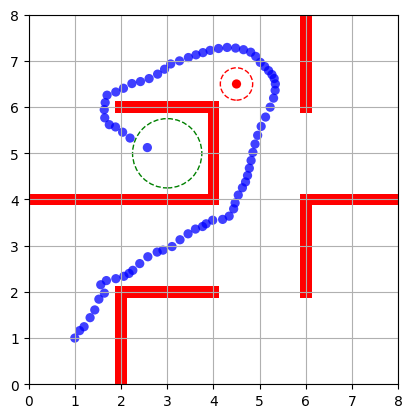
\includegraphics[scale=0.9]{img/image1.png}
\caption{Visualización de la trayectoria seguida por un robot simulado (punto azul) recorriendo un laberinto en presencia de un obstáculo dinámico (punto rojo).}
\end{figure}

\section{Resumen}
En el presente documento se presentan de forma sintética los fundamentos, implementación y resultados del trabajo realizado entre enero y junio del 2024, bajo supervisión del Dr. Israel Becerra Durán. Dicho trabajo estuvo enfocado en la planificación de movimiento de robots simulados en un entorno con obstáculos fijos y dinámicos. Partiendo del algoritmo de muestreo PRM (Probabilistic Roadmaps), ampliamente utilizado para planificar el movimiento de robots en entornos a priori desconocidos, se propone una variante que adapta el algoritmo para considerar la presencia de uno o más obstáculos dinámicos y posteriormente se explora la forma en que pueden aprovecharse las redes neuronales para automatizar el movimiento del robot, así como las estrategias de muestreo y entrenamiento utilizadas para incrementar la precisión de la red.

\newpage
%\vspace{50mm}
\section{Introducción}
En el campo de la robótica, la planificación de movimiento es una tarea crucial y el fundamento que permite a los robots navegar de manera eficiente y segura en diversos entornos. Los algoritmos de muestreo, como los Roadmaps Probabilísticos (PRM), objeto del enfoque de este proyecto, han demostrado ser herramientas poderosas en esta área, facilitando la generación de trayectorias viables en entornos complejos y con espacios de configuraciones de altas dimensiones. Estos algoritmos funcionan al crear una representación gráfica del espacio de configuraciones, donde los nodos representan configuraciones posibles y las aristas conectan estos nodos mediante movimientos factibles del robot.\\

Tradicionalmente, la mayoría de las aplicaciones de los algoritmos de muestreo se centran, al menos en su enfoque inicial, en entornos estáticos con obstáculos fijos. Sin embargo, el mundo real raramente es estático. Los entornos dinámicos, en los que los obstáculos pueden moverse y los robots pueden interactuar con otros robots o agentes antagonistas, presentan desafíos adicionales que requieren soluciones más avanzadas.\\

Integrar la capacidad de manejar obstáculos en movimiento y la presencia de robots antagonistas no solo aumenta la aplicabilidad de estos algoritmos en escenarios del mundo real, como almacenes automatizados, vehículos autónomos y robots de rescate, sino que también impulsa el desarrollo de sistemas más inteligentes y autónomos. Más aún, el rápido avance y accesibilidad de las redes neuronales para resolver rápidamente tareas de predicción nos brinda una excelente herramienta para agilizar y realizar en tiempo real la construcción de trayectorias correctas para un robot, a través del entrenamiento offline previo de estas redes.\\

Este proyecto pretende explorar cómo el algoritmo PRM puede ser adaptado para enfrentar la presencia de uno o varios obstáculos dinámicos, así como el potencial de integrar una red neuronal para predecir los pasos de la trayectoria del robot hacia un objetivo definido.


\section{Trabajo relacionado}
\subsection{Algoritmos de muestreo (PRMs)}
Los algoritmos de muestreo son técnicas fundamentales en la planificación de movimiento de robots, utilizados para explorar y mapear el espacio de configuraciones de un robot de manera eficiente. Los algoritmos más influyentes hasta el momento son los Probabilistic Roadmaps (PRMs) \cite{PRM} y los Rapidly-exploring Random Trees (RRTs) \cite{RRT}.\\

Los PRM funcionan creando una red de posibles trayectorias libres de colisión (roadmap) mediante la selección aleatoria de puntos en el espacio de configuraciones, conectando estos puntos con movimientos factibles y seguros para el robot. Una de las principales ventajas de los PRM es su flexibilidad y eficiencia en la generación de caminos, especialmente en entornos donde la configuración del espacio puede ser intrincada o parcialmente desconocida. Además, el PRM es un método \textit{multiple-query}, es decir, el mismo grafo puede ser utilizado para distintas posiciones iniciales y objetivo del robot.\\

De manera más técnica, definamos el problema de que un robot llegué a una región meta sin colisionar a través de la tripleta $(\mathcal{X}_{\text{free}}, x_{\text{init}}, \mathcal{X}_{\text{goal}})$, donde $\mathcal{X}_{\text{free}}$ es el espacio de configuraciones libre de obstáculos, $x_{\text{init}}$ es la configuración inicial del robot y $\mathcal{X}_{\text{goal}}$ es la región meta. Dado un $n\in \N$, el algoritmo PRM lo que hace es generar un grafo no dirigido $G = (V, E)$ donde $V \subset \mathcal{X}_{\text{free}}$, $card(V) \leq n+1$ y $E = V\times V$.\\

La forma en que se genera el grafo puede tener distintas implementaciones, algunas buscando un grafo acíclico, otras limitando las conexiones entre nodos, entre otras. En este proyecto, se consideró la variante de $sPRM$, referida en \cite{Optimal} una versión simplificada que genera un grafo que puede tener ciclos, pero en el cual podemos ajustar el radio de conexión $r$. El pseudocódigo se muestra en la Figura 3.1 y una visualización del proceso iterativo del algoritmo en la Figura 3.2.

\begin{figure}[hbtp]
\centering
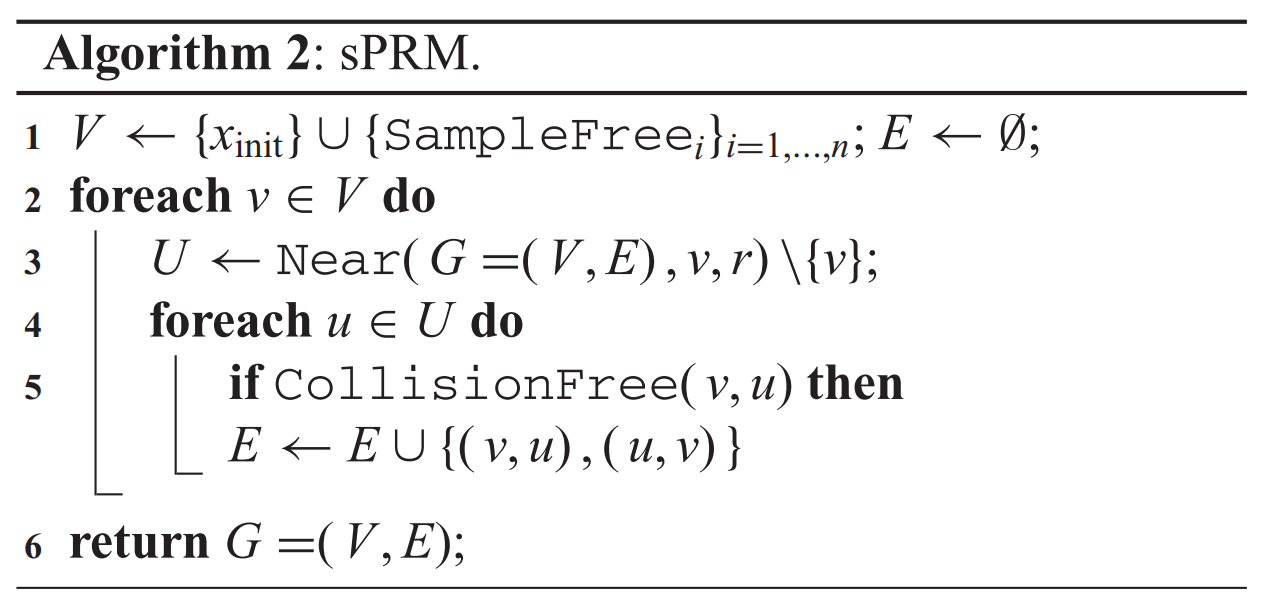
\includegraphics[scale=0.4]{img/sPRM pscode.png}
\caption{Pseudocódigo de sPRM, algoritmo tomado como base de este proyecto y extraído de \cite{Optimal}}
\end{figure}

Cabe resaltar que el algoritmo requiere de funciones auxiliares, que cumplen las siguientes tareas:
\begin{itemize}
\item \textbf{SampleFree}: Función booleana que nos dice si una muestra de configuración está libre de colisiones.

\item \textbf{Near}: Esta función regresa el conjunto de vértices del grafo (muestras) que se encuentran dentro de un radio $r$ de distancia (bajo alguna métrica) respecto a un vértice especificado (omitiendo dicho vértice).

\item \textbf{CollisionFree}: Esta función booleana determina si la línea que une dos configuraciones se encuentra libre de colisiones.
\end{itemize}
  \begin{figure}[hbtp]
\centering
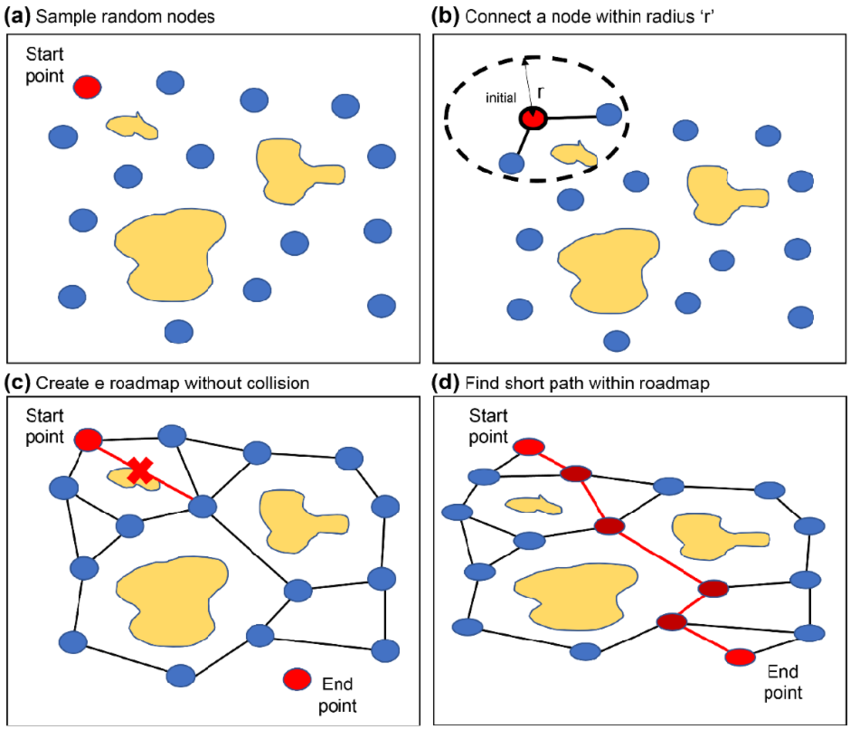
\includegraphics[scale=0.7]{img/PRM func.png}
\caption{Funcionamiento del algoritmo PRM}
\end{figure}


\subsection{Redes neuronales para predicción de trayectorias}
Entre los meses de junio y agosto del 2023 se realizó, igualmente bajo supervisión del Dr. Israel Becerra y en conjunto con otros compañeros, un análisis a los algoritmos de muestreo para planificación de movimiento óptima propuestos en \cite{Optimal}, seguido de la implementación de algunos relevantes como RRT, RRT*, PRM* y RRG.\\

El desarrollo y resultados de dicho proyecto se encuentra disponible en \cite{Verano}. Es pertinente mencionar que, además de la implementación de los algoritmos como tal, también se integró el uso de redes neuronales a través de la herramienta de TensorFlow, entrenadas para resolver el problema de predecir una configuración (en este caso, una posición en un entorno 2D) $x_{t+1}$ dado un estado $(x_t, x_{goal})$, donde en torno a $x_{goal}$ se define la región meta.\\

Las redes eran del tipo secuencial con capas densas y el entrenamiento se realizó gracias a la generación de archivos de texto que contenían trayectorias calculadas previamente bajo una serie de consideraciones de muestreo de puntos iniciales y puntos meta para cada trayectoria. Los detalles de esta estrategia, replicada y adaptada para la realización de este proyecto, se describen en la Sección 4.5.\\

Los resultados de la integración de las redes neuronales fueron satisfactorios, en el sentido de que permitieron comprobar la utilidad de estas redes para predecir trayectorias correctas y agilizaron el cálculo de estas a tiempos considerablemente más pequeños a que si se calculaban con algoritmos tradicionales de búsqueda en grafos (Figura 3.3).

\begin{figure}[hbtp]
\centering
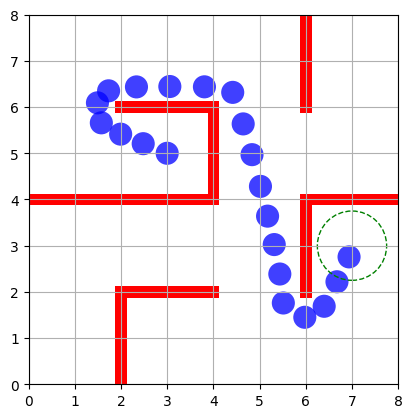
\includegraphics[scale=0.65]{img/MLPexample.png}
\caption{Ejemplo de trayectoria generada por un Multi-Layer Perceptron entrenado a partir de trayectorias de un RRT*}
\end{figure}

\section{Metodología e Implementación}
\subsection{Definición del problema}
Como se mencionó previamente, el principal problema a resolver cuando se utilizan algoritmos de muestreo es el de generar una trayectoria (entiéndase trayectoria como una secuencia de configuraciones) factible y libre de colisiones con obstáculos que lleve al robot desde una configuración inicial hasta una región meta en el espacio de configuraciones. No obstante, en este caso será necesario considerar que una trayectoria libre de colisiones evitará las colisiones con uno o varios osbtáculos dinámicos.\\

Para simplificar la definición del problema, supongamos que solamente tenemos un obstáculo dinámico. Si consideramos dos o más obstáculos dinámicos, la aproximación se puede extender de forma análoga.\\

Cuando consideramos la presencia del obstáculo dinámico se agrega al problema el factor del movimiento. Consecuentemente, a diferencia del problema con obstáculos fijos, tendremos que considerar un incremento de tiempo $\Delta t$ y una velocidad $v_{robot}$ y $v_{obst}$ para el robot y para el obstáculo dinámico, respectivamente. De esta manera, por cada paso de tiempo, tanto el robot como el obstáculo dinámico pueden moverse a lo más una distancia de $v_{robot}\Delta t$ y $v_{obst}\Delta t$ respectivamente.\\

Si bien un robot y un obstáculo dinámico pueden ser de diversas formas y tamaños, para el alcance de este proyecto supondremos que tanto el robot como el obstáculo dinámico son volúmenes esféricos en el espacio de configuraciones con radios $r_{robot}$ y $r_{obst}$. Con esto establecido, podemos definir una \textit{\textbf{región de alcanzabilidad}} del obstáculo dinámico, centrada en la posición de este y con un radio de 
$$reach_{obst} = v_{obst}\Delta t + r_{obst}$$ 
considerando el barrido del volumen del obstáculo. Si el robot se encuentra dentro de la región de alcanzabilidad del obstáculo dinámico, entonces se encuentra en peligro de colisionar con él en el actual o en el próximo instante de tiempo.\\

Con todo lo anterior, podemos sintetizar el problema a resolver como el de generar una secuencia de configuraciones 
$$(x_0, x_1, \dots, x_n)$$

tal que $x_0 = x_{init}$ es la configuración inicial del robot, $x_n$ se encuentra dentro de una región meta, i.e. $x_n \in \mathcal{X}_{goal}$  y en todo momento las configuraciones se encuentran libres de colisiones con los obstáculos fijos y fuera de la región de alcanzabilidad del obstáculo dinámico, es decir, 
$$x_i \in \mathcal{X}_{free} \Rightarrow distance(x_i, x_{obst_i}) > reach_{obst} \quad \forall 0\leq i \leq n$$

donde $x_i, x_{obst_i}$ son las configuraciones del robot y del obstáculo dinámico en el instante de tiempo $i$, considerando que $\Delta t$ se mantiene constante.\\

Cabe mencionar que la distancia entre dos posiciones consecutivas del robot y del obstáculo dinámico será de $v_{robot}\Delta t$ y $v_{obst}\Delta t$, respectivamente, ya que supondremos una velocidad constante para ambos. 

\subsection{Propuesta de adaptación al algoritmo PRM}
Ahora bien, para poder resolver el problema de planificación de movimiento descrito anteiormente, se propone utilizar el algoritmo sPRM, cuya estructura se muestra en la Figura 3.1. En este caso, la primera adaptación consiste en considerar el radio de conexión $r$ al llamar la función \textbf{Near} como 
$$r = v_{robot}\Delta t$$

dado que se considera que cualquier trayectoria que siga el robot constará de configuraciones separadas por esa distancia. Esto nos generará un grafo con nodos tales que sus vecinos inmediatos se encuentran a lo más a dicha distancia. La siguiente adaptación tiene que ver con el algoritmo que utilizamos una vez construido el grafo para obtener una trayectoria que lleve al robot a una región meta. Tradicionalmente, el algoritmo que obtiene tales trayectorias funciona con otro algoritmo de búsqueda óptima en grafos (como el algoritmo de Dijkstra) y está dado como se muestra en el Algoritmo 1.\\

Para generar una trayectoria considerando la posición y la región de alcanzabilidad del obstáculo dinámico en un tiempo determinado, se propone que el objeto \textit{vértice} del grafo del PRM cuente con un atributo que le permita activarse o desactivarse según sea el caso (esto puede implementarse en cualquier entorno de P.O.O.). De esta manera, se pretende \textit{\textbf{podar}} el grafo en torno a la región de alcanzabilidad del obstáculo dinámico y desactivar temporalmente aquellos vértices que se encuentren dentro de esta, para que cualquier trayectoria que se conecte con ellos no sea considerada en ese momento. Desde luego, el algoritmo de Dijkstra o cualquier otro de búsqueda en grafos que se utilicé tendría que considerar únicamente aquellos vértices y aristas que se encuentren activados. Así, el algoritmo de obtención de trayectorias estaría dado como se muestra en el Algoritmo 2.\\

Con todo lo anterior ya es posible encontrar trayectorias factibles al tener un obstáculo dinámico en un cierto instante de tiempo, como se muestra más adelante en la sección 4.3, sin embargo, se espera que el obstáculo dinámico se mueva constantemente y, con cada cambio de posición, será necesario estar recalculando las trayectorias. Esto, si bien es algo posible de hacer con los algoritmos presentados y con un poder de procesamiento razonable, en la mayoría de los casos es costoso computacionalmente e ineficiente. Por dicha razón, se propone utilizar una red neuronal para generar la trayectoria en tiempo real similar a las referidas en la Sección 3.2 y que logre ajustar la trayectoria de acuerdo a los cambios de posición del obstáculo dinámico.\\

Para entrenar la red neuronal, se generarán suficientes trayectorias utilizando el Algoritmo 2, considerando diversas posiciones para el obstáculo dinámico. De esta manera, dado un estado $(x_t, x_{obst}, x_{goal})$, donde $x_{obst}$ es la posición del obstáculo en el tiempo $t$ y en torno a $x_{goal}$ se define la región meta, se espera que la red pueda predecir una configuración $x_{t+1}$ que lleve acerque un poco más al robot hacia la meta. Los detalles de cómo será el entrenamiento en el alcance de este proyecto y los distintos factores a considerar se describirán más adelante en las secciones 4.4 y 4.5.
\newpage

\begin{algorithm}
\caption{Algoritmo tradicional para encontrar trayectorias}
\begin{algorithmic}[1]
\State \textbf{Entrada:} 
\State \hspace{\algorithmicindent} $G = (V, E)$: Grafo obtenido a partir del PRM
\State \hspace{\algorithmicindent} $x_{init}$: Configuración inicial
\State \hspace{\algorithmicindent} $x_{goal}$: Centro de la región meta
\State \hspace{\algorithmicindent} $r_{goal}$: Radio de la región meta
\State \textbf{Salida:} 
\State \hspace{\algorithmicindent} $PathV$: Camino de vértices (configuraciones) hacia la región meta.  
\State \hspace{\algorithmicindent} $PathE$: Camino de aristas (pares de vértices) hacia la región meta.
\vspace{3.5mm}
\Function{getPath}{$G, x_{init}, x_{goal}, r_{goal}$}
    \State $PathV, PathE \gets \text{Dijkstra}(G, x_{init}, x_{goal}, r_{goal})$
    \vspace{1.5mm}
    \If{$PathV = \textbf{None}$}
        \State \text{imprimir} "No hay trayectoria factible desde el punto de inicio al punto final."
    \EndIf
    \vspace{1.5mm}
    \State \Return $PathV, PathE$
\EndFunction
\end{algorithmic}
\end{algorithm}

\begin{algorithm}[h!]
\caption{Algoritmo para encontrar trayectorias dada la posición del obstáculo dinámico}
\begin{algorithmic}[1]
\State \textbf{Entrada:} 
\State \hspace{\algorithmicindent} $G = (V, E)$: Grafo obtenido a partir del PRM
\State \hspace{\algorithmicindent} $x_{init}$: Configuración inicial
\State \hspace{\algorithmicindent} $x_{goal}$: Centro de la región meta
\State \hspace{\algorithmicindent} $r_{goal}$: Radio de la región meta
\State \hspace{\algorithmicindent} $x_{obst}$: Configuración actual del obstáculo dinámico
\State \hspace{\algorithmicindent} $\lambda$: Factor de seguridad para omitir vértices muy cercanos (sin estar dentro) a la región de alcanzabilidad
\State \textbf{Salida:} 
\State \hspace{\algorithmicindent} $PathV$: Camino de vértices (configuraciones) hacia la región meta.  
\State \hspace{\algorithmicindent} $PathE$: Camino de aristas (pares de vértices) hacia la región meta.
\vspace{3.5mm}
\Function{getPathwObst}{$G, x_{init}, x_{goal}, r_{goal}, x_{obst}, \lambda$}
	\State $nearObst \gets \text{Near}(G, x_{obst}, reach_{obst} + \lambda)$
    \vspace{1.5mm}
    \ForAll{$v \in V$}
        \If{$v \in nearObst$}
            \State $v.\text{activate} \gets \text{False}$
        \EndIf
    \EndFor
    \vspace{1.5mm}
    \State $PathV, PathE \gets \text{Dijkstra}(G, x_{init}, x_{goal}, r_{goal})$
    \vspace{1.5mm}
    \If{$PathV = \textbf{None}$}
        \State \text{imprimir} "No hay trayectoria factible desde el punto de inicio al punto final."
    \EndIf
    \vspace{1.5mm}
   	\ForAll{$v \in V$}
        \State $v.\text{activate} \gets \text{True}$
    \EndFor
    \vspace{1.5mm}
    \State \Return $PathV, PathE$
\EndFunction
\end{algorithmic}
\end{algorithm}

\subsection{Definición del entorno de trabajo}
La implementación de este proyecto se llevó a cabo en el lenguaje de programación Python, mayoritariamente haciendo uso de Jupyter Notebook. Empezando por el \textit{workspace} donde estará el robot simulado, estaremos considerando un laberinto similar al presentado en la Sección 3.2, que consta de una cuadricula de $8 \times 8$ unidades con paredes con grosor de 0.25, como se muestra en la Figura 4.1.
\begin{figure}[hbtp]
\centering
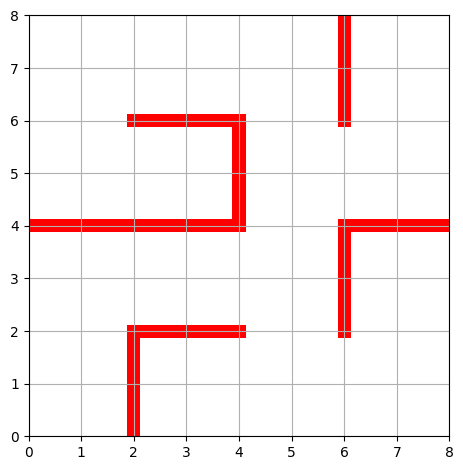
\includegraphics[scale=0.5]{img/maze.png}
\caption{Entorno 2D sobre el cual se desplazará el robot simulado.}
\end{figure}

Para el robot y el obstáculo dinámico, consideremos que ambos son robots circulares con radio de 0.1, es decir, 
$$r_{robot} = r_{obst} = 0.1$$

Además, supondremos 
$$v_{robot} = v_{obst} = 1$$

y un $\Delta t = 0.25$. De esta manera, el grafo resultante de ejecutar el PRM con todas las consideraciones anteriores y estableciendo 5000 muestras uniformemente se muestra en la Figura 4.2.
\begin{figure}[hbtp]
\centering
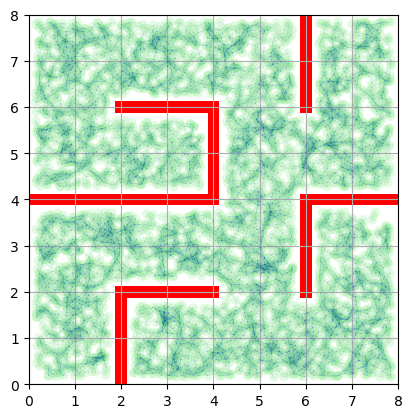
\includegraphics[scale=0.6]{img/PRMgraph.png}
\caption{Grafo resultante de ejecutar el algoritmo PRM}
\end{figure}
\newpage

A partir de este grafo, se implementaron también las funciones de los Algoritmos 1 y 2, para obtener trayectorias con y sin el obstáculo dinámico presente. Los resultados de una prueba realizada se muestran en la Figura 4.3.
\begin{figure}[!h]
  \centering
	{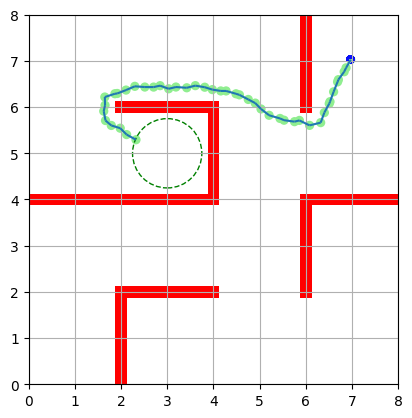
\includegraphics[width=0.45\textwidth]{img/path2.png}\label{fig:f1}}
  \hfill
  	{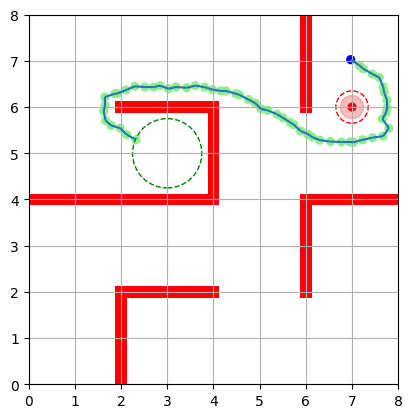
\includegraphics[width=0.45\textwidth]{img/pathObst.png}\label{fig:f2}}
  \caption{Trayectorias obtenidas sin obstáculo dinámico (izquierda) y con obstáculo dinámico (derecha). La región meta se delimita con el circulo punteado verde. El obstáculo dinámico es el punto rojo, las posiciones a las que puede moverse es la región roja sombreada y la región de alcanzabilidad se delimita con la circunferencia roja punteada (considerando el barrido del volumen del robot).}
\end{figure}

Sumado a todo lo anterior, se decidió subdividir el espacio del mapa $8 \times 8$ en 16 \textit{celdas} cuadriculares de $2 \times 2$ cada una (Figura 4.4), esto con el propósito de poder muestrear selectivamente posiciones del robot, región meta u obstáculo dinámico por celda, además de servir como base para los casos considerados a la hora de construir el conjunto de entrenamiento, como se expondrá en las siguientes dos secciones.
\begin{figure}[hbtp]
\centering
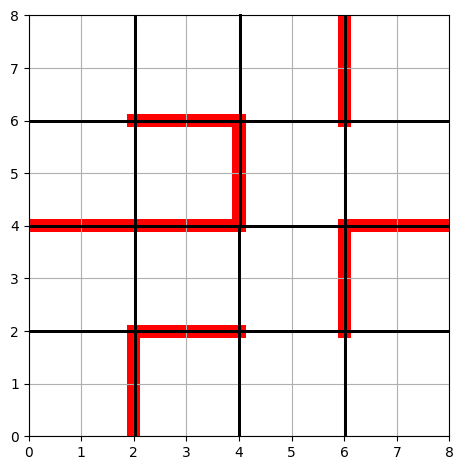
\includegraphics[scale=0.7]{img/cells.png}
\caption{Subdivisión del mapa en 16 celdas de $2 \times 2$ indexadas empezando desde la celda cero en la esquina inferior izquierda y siguiendo un orden de izquierda a derecha y después de abajo hacia arriba.}
\end{figure}

\subsection{Restricciones de implementación}
Como se mencionó previamente, un paso fundamental es la generación de trayectorias con la mayor cantidad de muestras posibles, con el fin de servir como entrenamiento para una red neuronal secuencial. Una aproximación inicial sugiere considerar una buena cantidad de entre todos los casos posibles ubicando la posición inicial del robot, la región meta y al obstáculo dinámico a lo largo de todas las celdas del mapa. No obstante, considerar todos estos casos plantea un problema de costo y tiempo de cálculo requerido, y para ejemplificarlo supongamos que deseamos calcular todas las trayectorias posibles considerando 5 posiciones iniciales del robot en cada celda, 10 del obstáculo dinámico en cada celda y establecer la región meta en el centro de cada celda, excluyendo la inicial para el robot, según sea el caso. Para ello tendríamos que generar un total de 
$$(16\times 5)\times(16 \times 10)\times 15 = 192000$$

trayectorias, que en promedio tardan unos 3 segundos en calcularse (dado el equipo de cómputo utilizado durante el proyecto), por lo que representaría una gran cantidad de tiempo, aunado a que el entrenamiento aún así no lograría una precisión muy alta para que la red prediga correctamente en tiempo real (como se verá en la sección 5). Por dichas razones, y con el objetivo de enfocarnos más en que la red pueda predecir correctamente la trayectoria con el obstáculo dinámico moviéndose, se decidió restringir (por el momento) las trayectorias a considerar para el entrenamiento.\\

Es así que, para las trayectorias utilizadas para el entrenamiento, al menos en esta etapa temprana del proyecto, se consideró una posición inicial del robot fija en $[1, 1]$ y como celda meta se eligió la número 9, centrada en $[3, 5]$. Como se mencionó previamente, se busca priorizar el entrenamiento de la red para actuar ante el movimiento constante del obstáculo dinámico, por lo cual para este consideraremos una cantidad $n$ de posiciones por cada una de las 16 celdas del mapa, empezando desde $n=15$ y hasta $n=30$, con el fin de evaluar la cantidad óptima de posiciones requeridas para un funcionamiento eficiente del modelo. 

\subsection{Construcción del conjunto de entrenamiento}

A grandes rasgos, el conjunto de entrenamiento consiste en archivos de texto donde para cada fila se guarda una trayectoria correspondiente a un caso con un punto inicial, un centro de región meta y una posición de obstáculo dinámico. Como se estableció previamente, el punto inicial y el meta serán fijos en esta ocasión, y lo que irá variando son las posiciones de obstáculo dinámico.\\

La forma en que se procedió fue considerando 15, 20, 25 y 30 posiciones aleatorias del obstáculo dinámico por celda del mapa. De esta forma, para cada muestra se generó una trayectoria que posteriormente sería guardada en el archivo de texto, usado más adelante para entrenar la red.


\subsubsection{Muestreo para el obstáculo dinámico}
Inicialmente, se consideró generar las posiciones del obstáculoo dinámico de forma aleatoria, siguiendo una distribución uniforme, sin embargo, como se verá en las siguientes imágenes, al generarlas de esta forma podía suceder que se formaran ciertos ''huecos'' o por otro lado ''islas'' de posiciones a lo largo del mapa, dejando algunas regiones, aunque pequeñas, sin considerar para el entrenamiento.\\

Por dicha razón, se implementó una función para distribuir de mejor manera las posiciones manteniendo la aleatoriedad. Tal función, al generar una muestra aleatoria, evalúa si se encuentra demasiado cerca de otras posiciones generadas y toma eso en cuenta para agregarla o rechazarla. Esto permite tener una mejor dispersión de las posiciones aleatorias del obstáculo dinámico a lo largo de todas las celdas.

\begin{figure}[hbtp]
\centering
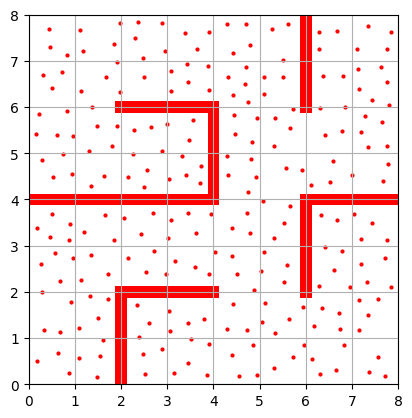
\includegraphics[scale=0.7]{img/15.png}
\caption{Posiciones de obstáculo dinámico consideradas para las trayectorias en el caso $n=15$ posiciones por celda.}
\end{figure}

\begin{figure}[h!]
\centering
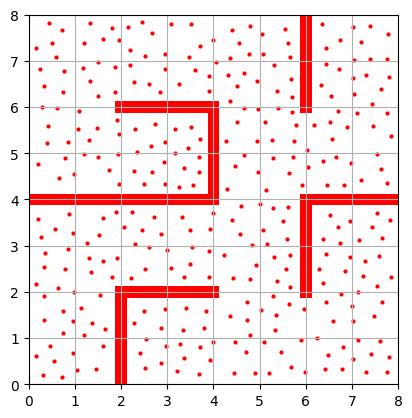
\includegraphics[scale=0.7]{img/20.png}
\caption{Posiciones de obstáculo dinámico consideradas para las trayectorias en el caso $n=20$ posiciones por celda.}
\end{figure}
\newpage

\begin{figure}[!h]
  \centering
	{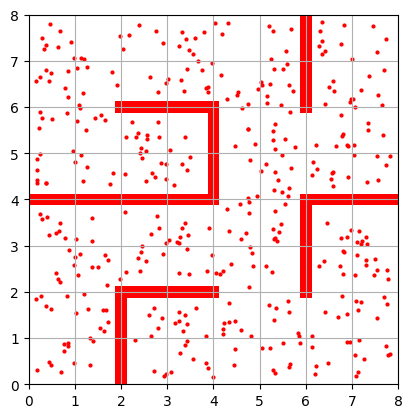
\includegraphics[width=0.45\textwidth]{img/25alt.png}\label{fig:f1}}
  \hfill
  	{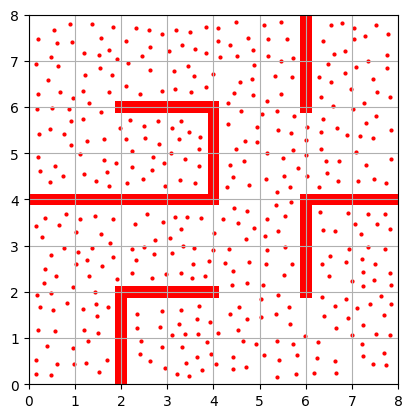
\includegraphics[width=0.45\textwidth]{img/25.png}\label{fig:f2}}
  \caption{Posiciones de obstáculo dinámico consideradas para las trayectorias en el caso $n=25$ posiciones por celda. Se incluye una comparativa de posiciones generadas aleatorialente (izquierda) que muestra la necesidad de usar una función que disperse de mejor forma las muestras.}
\end{figure}

\begin{figure}[h!]
\centering
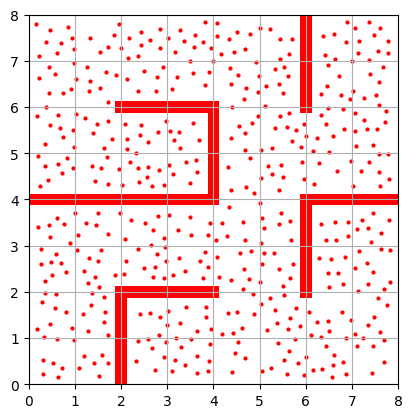
\includegraphics[scale=0.7]{img/30.png}
\caption{Posiciones de obstáculo dinámico consideradas para las trayectorias en el caso $n=30$ posiciones por celda.}
\end{figure}


Una vez creados los archivos con las trayectorias, para cada uno de los casos se creo un dataframe en pandas en donde cada trayectoria, que para entonces consistía en una fila ordenada de pares de números, se descompuso en pares del tipo
$$
\left[ (x_t, x_{obst}, x_{goal}), (x_{t+1})\right],
$$

cada elemento del par ubicado en una columna del dataframe. Este dataframe se utilizó en cada caso para entrenar una red secuencial construida en Tensorflow con 3 capas ocultas más la capa de entrada y la capa de salida. En todas las redes se utilizaron 1000 épocas para el entrenamiento. 

\newpage
\section{Resultados}
Al correr los modelos entrenados con algunos casos de prueba en cuanto a la posición del obstáculo dinámico se vieron resultados como los siguientes.
\begin{figure}[!h]
  \centering
	{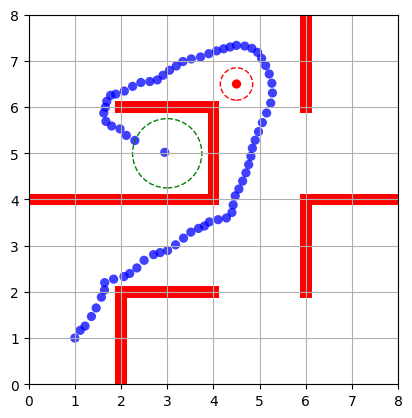
\includegraphics[width=0.3\textwidth]{img/win1.png}\label{fig:f1}}
  \hfill
  	{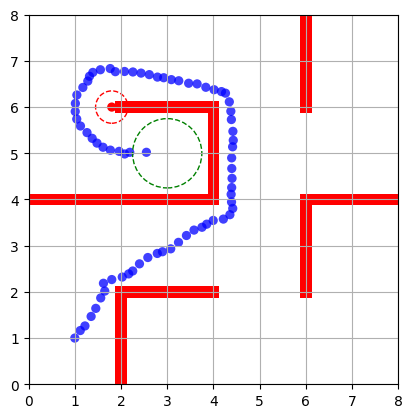
\includegraphics[width=0.3\textwidth]{img/win2.png}\label{fig:f2}}
  	\hfill
  	{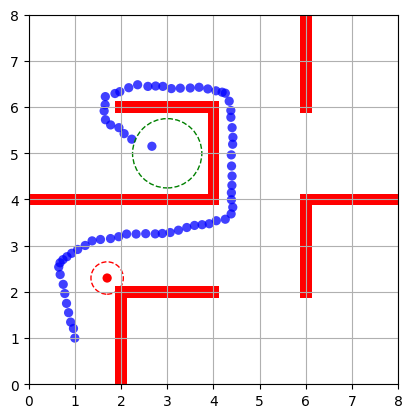
\includegraphics[width=0.3\textwidth]{img/win3.png}\label{fig:f3}}
  \caption{Casos de prueba a las redes exitosos.}
\end{figure}

Sin embargo, también se tuvieron casos como los siguientes.
\begin{figure}[!h]
  \centering
	{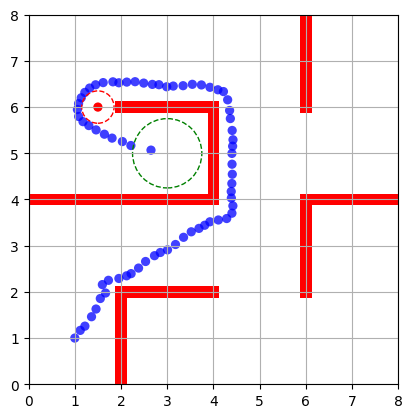
\includegraphics[width=0.3\textwidth]{img/loss1.png}\label{fig:f1}}
  \hfill
  	{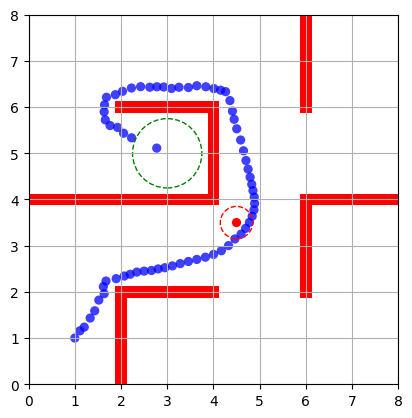
\includegraphics[width=0.3\textwidth]{img/loss2.png}\label{fig:f2}}
  	\hfill
  	{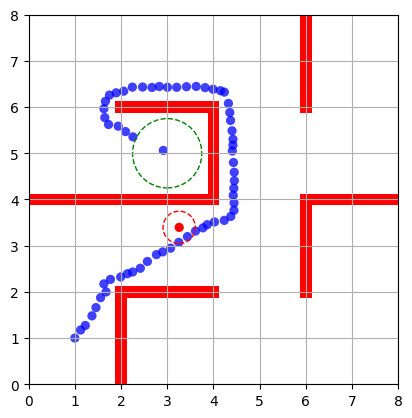
\includegraphics[width=0.3\textwidth]{img/loss3.png}\label{fig:f3}}
  \caption{Casos de prueba a las redes no exitosos.}
\end{figure}


Por dicha razón, con el fin de evaluar el desempeño de los modelos en condiciones similares y particularmente, ver cuál fue la mejor selección de número de posiciones de obstáculo por celda entre las que se consideraron, se generaron 20 posiciones de obstáculo aleatorias a lo largo de todo el mapa, para posteriormente evaluarlas para cada uno de los modelos y contar el número de trayectorias exitosas. Una trayectoria se dice exitosa si en ningún momento el robot colisionó con algún obstáculo fijo, se mantuvo fuera de la región de alcanzabilidad del obstáculo dinámico y llegó a la región objetivo. A continuación se presenta una tabla comparativa de los modelos evaluados. El nombre de cada modelo hace referencia a las consideraciones tomadas para generar las trayectorias con las que fue entrenado.
\newpage

\begin{center}
\begin{tabular}{|l|c|c|}
\hline
\multicolumn{1}{|c|}{\textbf{Modelo}}                                                                                 & \textbf{\begin{tabular}[c]{@{}c@{}}Número de \\ trayectorias exitosas\\ (de 20 totales)\end{tabular}} & \textbf{\% de éxito} \\ \hline
\begin{tabular}[c]{@{}l@{}}15 posiciones de obstáculo \\ dinámico por celda\\ (completamente aleatorias)\end{tabular} & 15                                                                                                    & 75\%                 \\ \hline
\begin{tabular}[c]{@{}l@{}}15 posiciones de obstáculo\\ dinámico por celda\\ (aleatorias dispersadas)\end{tabular}    & 15                                                                                                    & 75\%                 \\ \hline
\begin{tabular}[c]{@{}l@{}}20 posiciones de obstáculo\\ dinámico por celda\\ (completamente aleatorias)\end{tabular}  & 16                                                                                                    & 80\%                 \\ \hline
\begin{tabular}[c]{@{}l@{}}20 posiciones de obstáculo\\ dinámico por celda\\ (aleatorias dispersadas)\end{tabular}    & 14                                                                                                    & 70\%                 \\ \hline
\begin{tabular}[c]{@{}l@{}}25 posiciones de obstáculo\\ dinámico por celda\\ (completamente aleatorias)\end{tabular}  & 17                                                                                                    & 85\%                 \\ \hline
\begin{tabular}[c]{@{}l@{}}25 posiciones de obstáculo\\ dinámico por celda\\ (aleatorias dispersadas)\end{tabular}    & 18                                                                                                    & 90\%                 \\ \hline
\begin{tabular}[c]{@{}l@{}}30 posiciones de obstáculo\\ dinámico por celda\\ (completamente aleatorias)\end{tabular}  & 15                                                                                                    & 75\%                 \\ \hline
\begin{tabular}[c]{@{}l@{}}30 posiciones de obstáculo\\ dinámico por celda\\ (aleatorias dispersadas)\end{tabular}    & 16                                                                                                    & 80\%                 \\ \hline
\end{tabular}
\end{center}

\vspace{1.5mm}

Como se puede observar, parece ser que considerar las posiciones del obstáculo dinámico más dispersadas si influyó en mejorar el desempeño de la red entrenada bajo esta consideración. Además, vemos que el mejor desempeño se logró con la red entrenada con trayectorias con posiciones de obstáculo dinámico dispersadas y de 25 por celda del mapa. Posiblemente la baja en el desempeño en comparación con los modelos de 30 posiciones por celda se deba a un ligero sobreajuste presente en el entrenamiento de estos últimos.\\

Ahora bien, un punto fundamental y el objetivo del proyecto es el de probar el modelo en un entorno dinámico. Por dicha razón, se selecconó el modelo con mejor desempeño (25 posiciones dispersadas) y se plantearon diversos escenarios con el obstáculo dinámico moviéndose, siguiendo un patron establecido, por ejemplo, moverse a lo largo de un pasillo o una celda. Posteriormente se generó una animación en matplotlib para estos casos, cuyos resultados, en general exitosos, se pueden visualizar en la siguiente liga.


\begin{itemize}
\item \url{https://drive.google.com/drive/folders/1KGqsj2VFKTCNakIvL3H2wOmrSfs9qko_?usp=sharing}
\end{itemize}



\subsection{Limitaciones y posibles mejoras}
La principal limitación del modelo desde luego está en las restricciónes que se consideraron para esta primera etapa de implementación del proyecto. El hecho de que haya un inicio y un final fijo restringe el panorama a solo estos casos particulares. En futura investigación, se pretende extender los casos a puntos de inicio y objetivo en todas las celdas del mapa, siempre que se tenga el equipo de cómputo necesario.\\

Otra importante limitación y un tanto problemática que presentan los modelos, incluso el que tuvo mejor desempeño, es que la red es incapaz de anticiparse demasiado a los movimientos del obstáculo dinámico, es decir, puede encaminarse a una trayectoria que para el momento es segura pero que unos instantes puede estar bloqueada por el obstáculo dinámico. Para cuando llega ese instante, la red también tiene dificultad en corregir el curso de la trayectoria rápidamente, por lo que en la mayoría de estas ocasiones termina colisionando. Un ejemplo de este problema se encuentra en la siguiente liga.

\begin{itemize}
\item \url{https://drive.google.com/file/d/1Z6W93jAMDWmxbF5T7pgolaI1XjEkNokh/view?usp=sharing}
\end{itemize}

Curiosamente, al reducir la velocidad del obstáculo dinámico, el robot si es capaz de anticiparse y seguir una trayectoria segura, como se muestra a continuación.

\begin{itemize}
\item \url{https://drive.google.com/file/d/1U15uxr5Bzi3MZinAY2C63OJXc9Pl52CS/view?usp=sharing}
\end{itemize}

Una posible solución a este problema es también una solución a la primera limitación presentada, que es extender el número de posiciones, particularmente las iniciales, a todas las celdas del mapa, además de considerar más posiciones de obstáculo por celda. Esto en teoría permitiría a la red considerar rutas alternas a la meta más allá de las que sigue comunmente desde un punto inicial fijo, y de esta manera corregir de mejor manera el curso de trayectorias a punto de colisionar. Además de ello, es relevante mencionar que una conclusión a la que se llegó durante la realización del proyecto \cite{Verano} fue que algoritmos como el PRM (con radio de conexión suficientemente pequeño) o RRT* tienden a generar trayectorias con optimalidad. Este factor puede ser bueno si lo que se busca es seguir el camino más corto, sin embargo, estas trayectorias tienden a acercar el robot a las orillas de los obstáculos y, en este caso, a la región de alcanzabilidad. Una alternativa sería considerar algoritmos no óptimos, como el RRT, los cuales construyen caminos con mayor libertad de correción de curso y que alejan más al robot de zonas potencialmente peligrosas.   

\section{Conclusiones}
En este proyecto, hemos explorado una variante del algoritmo de planificación de movimiento PRM complementado con redes neuronales para la planificación de movimiento. Los resultados obtenidos han sido en su mayoría satisfactorios, demostrando que la integración de redes neuronales con la variante del PRM presentada puede contribuir de buena manera en la generación en tiempo real de trayectorias seguras y óptimas para el robot.\\

No obstante, se han identificado ciertas limitaciones que requieren atención futura. Entre ellas, la necesidad de una mayor robustez ante los movimientos rápidos del obstáculo dinámico y la de extender los casos considerados para el entrenamiento. A pesar de estas limitaciones, el proyecto tiene un claro potencial para seguir extendiéndose y mejorándose. La ruta de investigación futura incluye los siguientes puntos.

\begin{itemize}
\item Extensión de los casos de entrenamiento.
\item Consideración de otros algoritmos no óptimos como RRT.
\item Presencia de más obstáculos dinámicos.
\item Dotar al obstáculo dinámico de un modelo similar al del robot, que permita planificar sus movimientos e involucre un escenario de juego cooperativo, donde ambos busquen no colisionarse mutuamente. 
\item Extensión a espacios de configuraciones de mayor dimensión.
\end{itemize}

En conclusión, la integración de algoritmos de muestreo en conjunto con redes neuronales representa un paso significativo hacia la planificación de movimiento más eficiente y adaptable en entornos dinámicos. Con mejoras y ajustes continuos, esta línea de investigación promete contribuir de manera sustancial al campo de la robótica y la inteligencia artificial. 

\newpage
\begin{thebibliography}{9}
    \bibitem{PRM}
    Kavraki LE, Svestka P, Latombe JC and Overmars MH,
    \emph{Probabilistic roadmaps for path planning in high-dimensional
configuration spaces} (1996),
    IEEE Transactions on Robotics and Automation.

    \bibitem{RRT}
    LaValle SM,
    \emph{Planning Algorithms} (2006),
    Cambridge University Press.
    
    \bibitem{Optimal}
    Karaman S and Frazzoli E,
    \emph{Sampling-based algorithms for optimal motion planning} (2011),
    The International Journal of Robotics Research.
    
    \bibitem{Verano}
    Guajardo LR, Castañeda J, Suro AA, Paz MA,
    \emph{Redes Neuronales y Algoritmos de Planificación} (2023),
    disponible en \href{https://github.com/RamonGuajardo1017/Robotics-Summer-2023}{Robotics-Summer-2023}
\end{thebibliography}

\end{document}